% !TEX encoding = UTF-8 Unicode
% -*- coding: UTF-8; -*-
% vim: set fenc=utf-8
\section{PT ISIM}
PT ISIM обеспечивает непрерывный мониторинг сетевой активности и позволяет выявлять уязвимости и хакерские атаки на промышленную сеть предприятия. PT ISIM не оказывает влияния на технологический процесс, сетевую инфраструктуру и промышленное оборудование, поскольку подключается однонаправленным способом, физически исключающим какое-либо воздействие.\par

PT ISIM использует для анализа копию трафика технологической сети, детектирует события кибербезопасности и выявляет связи между ними. Интеллектуальная система корреляции событий позволяет PT ISIM обнаруживать нелегитимные действия нарушителя и представлять их в виде наглядной цепочки шагов развития атаки (в том числе потенциальной). Уникальные возможности визуализации инцидентов в PT ISIM помогают оперативно определять векторы распределенных во времени атак и соотносить их с элементами как сетевой инфраструктуры, так и технологического процесса промышленного объекта. Кроме того, сохраненная копия трафика позволяет в любой момент провести ретроспективный анализ и расследование инцидента.\par

PT ISIM помогает бороться с различными угрозами безопасности, включая несанкционированное подключение к сети, подбор паролей к компонентам системы, неправомерное исполнение управляющих команд, подмену проектов ПЛК и прошивок промышленного оборудования. PT ISIM позволяет выявлять и внутренние угрозы, такие как потенциально опасные действия персонала и ошибки конфигурации.\par

В состав решения на базе PT ISIM также входит набор компонентов, необходимых для организации центра оперативного управления комплексной распределенной системой промышленной кибер- безопасности (security operation center, SOC).\par

\clearpage

\begin{figure}[h!]
    \centering
    \includegraphics[width=1\textwidth]{04}
    \caption{Пример развертывания PT ISIM}
    \label{img:04}
\end{figure}

\subsection{Ключевые возможности}
­Безопасность технологического процесса. Архитектура пассивного мониторинга PT ISIM исключает нежелательное воздействие на технологический процесс.\par

Контроль целостности сети. PT ISIM автоматически инвентаризирует элементы сети, включая компоненты промышленной системы управления, и непрерывно контролирует целостность технологической сети.\par

­Визуализация инцидентов. За счет удобных средств графического отображения элементов сетевой топологии и технологического процесса (мнемосхемы), можно визуализировать инциденты информационной безопасности, в том числе на уровне бизнес-логики.\par

Обнаружение сложных атак. PT ISIM анализирует события информационной безопасности и связывает их в логические цепочки. Цепочка событий позволяет наглядно представить развитие инцидента во времени и в нужный момент принять соответствующие меры по предотвращению угрозы. Таким образом, PT ISIM эффективно выявляет и длительные многоэтапные атаки.\par

Оперативное реагирование на инциденты ИБ. В случае возникновения инцидента PT ISIM предоставляет ответственным сотрудникам информацию, соответствующую их полномочиям. Оперативный персонал располагает минимальным набором инструментов, необходимых для поддержки административных регламентов, а служба ИБ получает полный доступ к информации об инцидентах для их расследования.\par

Учет специфики предприятия. С помощью PT ISIM можно контролировать векторы атак, уникальные для промышленного объекта. Для настройки механизма контроля этих векторов используются данные, получаемые в результате анализа защищенности АСУ ТП предприятия.\par

Соответствие требованиям промышленной среды. Физические условия эксплуатации в промышленности бывают крайне агрессивными. Промышленное исполнение PT ISIM подбирается с учетом специфики отрасли и защищаемого предприятия.\\

\subsection{Назначение системы}

Система PT ISIM предназначена для повышения уровня защищенности, доступности и поддержки непрерывности технологических процессов с помощью анализа сетевого трафика и превентивного обнаружения атак, направленных на АСУ ТП.\par

Цели построения системы:
\begin{itemize}
    \item­ непрерывный анализ киберзащищенности АСУ ТП;
    \item контроль действий персонала и подрядчиков;
    \item обнаружение нарушений ИБ и кибератак на АСУТП;
    \item своевременное выявление инцидентов и информирование ответственных лиц;
    \item создание доверенного источника данных для эффективного проведения расследований нарушений ИБ;
    \item анализ инцидентов, включая определение причин возникновения, а также оценку последствий;
    \item помощь в планировании мер по устранению и предотвращению инцидентов;
    \item обеспечение соответствия требованиям регулирующих организаций (в том числе выполнение приказа ФСТЭК №31, норм закона о КИИ и выстраивание взаимодействия с центрами системы ГосСОПКА).
\end{itemize}

Задачи, решаемые PT ISIM:
\begin{itemize}
    \item непрерывная обработка копии трафика АСУ ТП, получаемого через однонаправленный шлюз (диод данных);
    \item анализ событий на уровне различных коммуникационных протоколов, включая промышленные (S7, Modbus, IEC);
    \item автоматическая визуализация схемы сети АСУТП;
    \item выявление неавторизованных подключений к сети АСУ ТП;
    \item детектирование потенциальных угроз и прямых попыток эксплуатации известных уязвимостей;
    \item обнаружение неавторизованного изменения технологических параметров;
    \item контроль доступа к настройкам ПЛК по сети (чтение и изменение микропрограмм и проектов ПЛК);
    \item обнаружение неавторизованного управления ПЛК по сети;
    \item выявление сложных, распределенных во времени атак на АСУ ТП (цепочки атак);
    \item генерация инцидентов ИБ с учетом логики технологического процесса;
    \item визуализация мнемосхемы техпроцесса и индикация компонентов, работа которых нарушена в результате инцидентов ИБ;
    \item формирование и отправка информации об инцидентах и состоянии защищенности АСУ ТП во внешние системы (SIEM, ГосСОПКА).\\
\end{itemize}

\subsection{Возможности масштабирования}
Решение на базе PT ISIM гибко масштабируется в зависимости от конкретных требований и задач. Внедрение компонентов PT ISIM может происходить поэтапно, не требуя крупных единовременных инвестиций. Базовая версия сетевого сенсора -- PT ISIM Traffic View Server -- требует минимальных усилий по установке и идеально подходит как для пилотного внедрения, так и для каждодневной эксплуатации. В дальнейшем опции лицензирования PT ISIM позволяют расширять функциональность системы без замены оборудования. Итоговое количество компонентов PT ISIM в составе системы не ограничено. На начальных этапах развертывания система может использоваться только на критически важных площадках с последующим полным покрытием всех процессов в сети промышленных объектов.\par

\begin{figure}[h!]
    \centering
    \includegraphics[width=1\textwidth]{05}
    \caption{Пример внедрения PT ISIM с минимальными затратами}
    \label{img:05}
\end{figure}

\clearpage

\begin{figure}[h!]
    \centering
    \includegraphics[width=1\textwidth]{06}
    \caption{Пример внедрения PT ISIM для максимальной эффективности}
    \label{img:06}
\end{figure}

\subsection{Структура}
Система PT ISIM представляет из себя программно-аппаратный комплекс, включающий серверы анализа сетевого трафика (сенсоры), серверы бизнес-аналитики и управления уровня ситуационного центра (SOC), а также панельный компьютер, предназначенный для индикации и квитирования критически опасных инцидентов оперативным персоналом промышленных объектов.\par

На уровне защищаемого сетевого сегмента АСУ ТП (в котором расположены АРМ операторов, серверы SCADA и ПЛК) применяются серверы сбора и анализа трафика -- сенсоры, View Servers. Они получают копию трафика с порта зеркалирования коммутатора (Mirror/SPAN) или TAP-устройства. При этом между сегментом АСУ ТП и сенсором устанавливается аппаратный однонаправленный шлюз данных (data diode) для исключения влияния PT ISIM на действующий технологический процесс.\par

Для организации ситуационного центра используются компоненты Overview Server (сводная информация о зарегистрированных инцидентах), Forensic Server (расследование инцидентов) и Management Server (централизованная настройка и обновление компонентов системы).\par

Все компоненты работают под управлением ОС Debian. Взаимодействие между всеми компонентами PT ISIM производится по протоколу HTTPS. Для установки и первоначальной настройки может требоваться доступ по протоколу SSH.\par

Для серверов-сенсоров (View Servers) доступны четыре вида шасси в зависимости от физических условий эксплуатации. Заказчик может выбрать любой из них. Допускается обновление ранее приобретенной лицензии PT ISIM View Server до более функциональной (при этом не требуется замена аппаратного шасси).\par

Конечные пользователи (инженеры по кибербезопасности) работают со всеми компонентами PT ISIM через современный браузерный веб-интерфейс по защищенному соединению (HTTPS).\\

\subsection{Компоненты PT ISIM}

\begin{figure}[h!]
    \centering
    \includegraphics[width=1\textwidth]{07}
    \caption{Компоненты PT ISIM}
    \label{img:07}
\end{figure}

PT ISIM View Server:
\begin{itemize}
    \item анализ копии трафика сегмента АСУ ТП;
    \item обработка событий в реальном времени;
    \item поддержка промышленных и IT-протоколов (DPI);
    \item автоматическая идентификация узлов;
    \item визуализация топологии промышленной сети;
    \item интеллектуальное обнаружение нарушений ИБ;
    \item анализ событий с учетом бизнес-логики техпроцесса;
    \item мощный ретроспективный анализ событий.
\end{itemize}

\begin{figure}[h!]
    \centering
    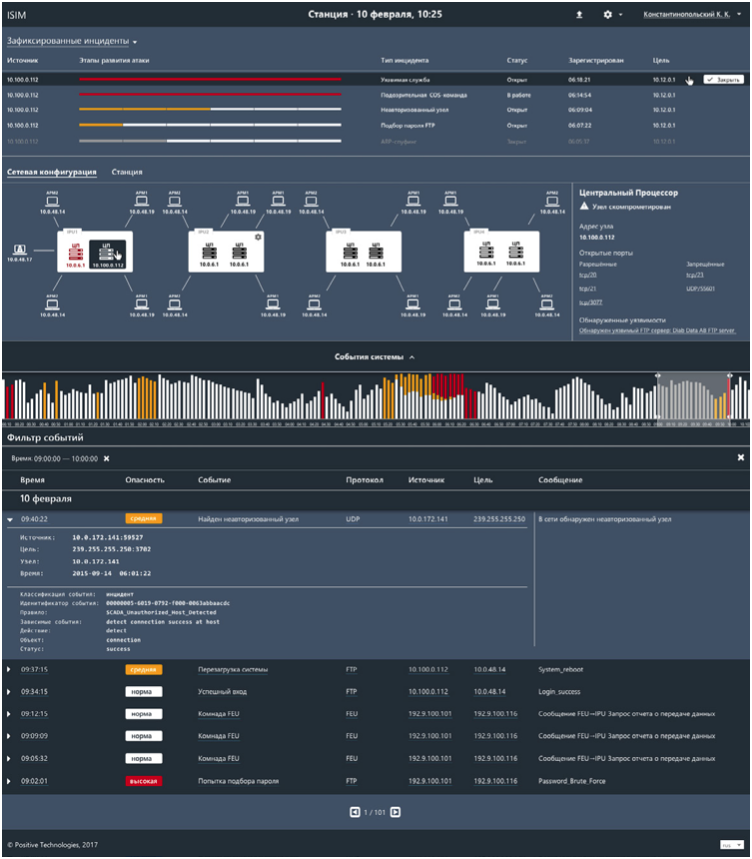
\includegraphics[width=1\textwidth]{08}
    \caption{Пользовательский интерфейс View Server}
    \label{img:08}
\end{figure}

PT ISIM OverView Server:
\begin{itemize}
    \item агрегация данных об инцидентах, поступающих с нескольких сенсоров (View Servers);
    \item визуализация сводной информации о защищенности (бизнес-аналитика);
    \item базовый анализ инцидентов и поддержка принятия оперативных решений;
\end{itemize}

PT ISIM Forensic Server:
\begin{itemize}
    \item агрегация полного объема данных для расследования инцидентов, включая необходимые копии трафика с сенсоров;
    \item управление инцидентами (жизненный цикл);
    \item моделирование инцидентов с учетом актуальной на тот момент конфигурации системы;
    \item­ импортирование данных об инцидентах с внешнего носителя.
\end{itemize}

PT ISIM Management Server:
\begin{itemize}
    \item управление параметрами компонентов PT ISIM;
    \item обновление компонентов PT ISIM;
    \item комплексная диагностика.
\end{itemize}

PT ISIM Industrial Tablet:
\begin{itemize}
    \item вывод информации о критически опасных инцидентах, требующих от оперативного персонала промышленного объекта немедленного реагирования в соответствии с регламентами;
    \item экспорт данных об инцидентах на внешний носитель.
\end{itemize}